% Provenance (never printed): old premiere S material on plate kinematics (rigid
% plates, rates from magnetic anomalies and from satellite positioning, hotspots
% and the Hawaiian chain, the coherence of the model); see
% sources/book2/PROVENANCE.md. Velocities from the NNR-MORVEL56 poles
% (figdata/grade-11/plate_velocities.py), station series from the Nevada Geodetic
% Laboratory (gnss_series.py), volcano ages from Clague and Dalrymple 1987
% (hawaii_chain.py). Euler poles and triple junctions belong to Year 1: the
% rotation pole is told, not defined.
\chapter{Plates and Their Motions}\label{ch:g11:plate-motions}

Near the summit of Mauna Kea, on the island of Hawaii, an antenna fixed to the
rock has been receiving the signals of positioning satellites every day since
October 1996. Each day a computer works out where the antenna is, to a few
millimetres. Thirty years of positions tell the same story every year: the
antenna, the mountain and the whole island move about \qty{7}{cm} a year
toward the west-north-west, without stopping and without turning. By 2026 the
antenna stood more than two metres from where it started. This chapter
measures such motions, shows how they fit together on a sphere, and reads the
same motion in the chain of dead volcanoes that stretches from Hawaii across
the northern Pacific.
% ledger: data:b2-ngl-gnss

\begin{recall}
The \omterm{def:g11:lithosphere-asthenosphere:lithosphere}{lithosphere} is broken into tectonic plates that move relative to each
other at a few centimetres a year; their boundaries are ridges, trenches,
collision zones and transform faults (Book 1, grade 7). A hotspot is a place
deep in the mantle that feeds a volcano on the plate above it; the plate
carries the volcano away while a new one grows over the hotspot (Book 1,
grade 7). A satellite-positioning receiver works out its own position from
the signals of several satellites (Book 1, grade 9). The magnetic stripes of
the ocean floor give the \omterm{def:g11:drift-to-spreading:spreading-rate}{spreading rate} of a ridge
(\cref{ch:g11:drift-to-spreading}), and the \omterm{def:g11:lithosphere-asthenosphere:lithosphere}{lithosphere} is the rigid outer
shell of the Earth, about \qty{100}{km} thick
(\cref{ch:g11:lithosphere-asthenosphere}). A speed of \qty{1}{cm} a year is
\qty{10}{km} per million years, and \qty{1}{mm} a year is \qty{1}{km} per
million years.
\end{recall}

\begin{omfigure}
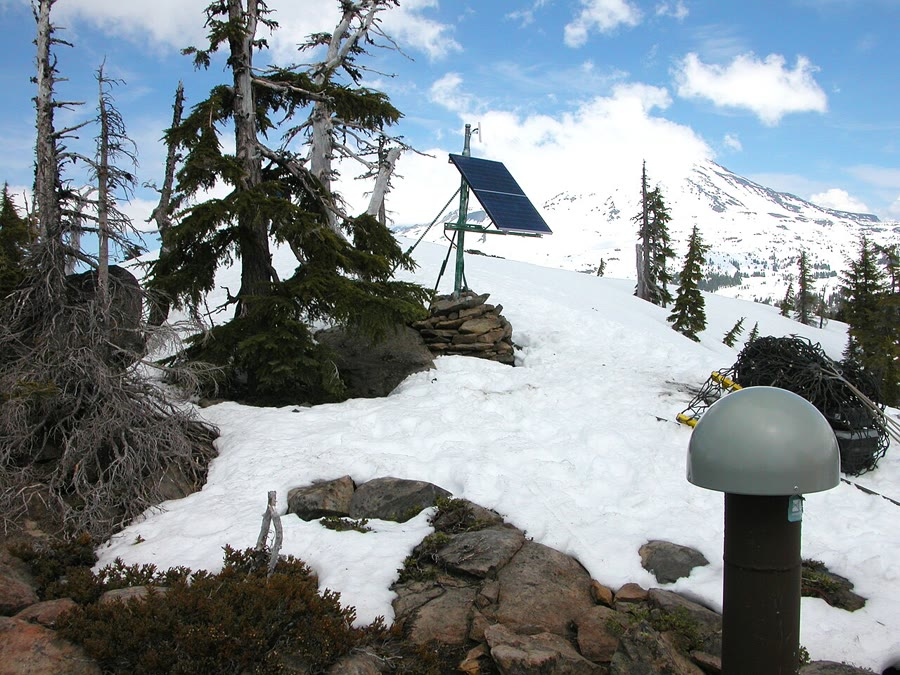
\includegraphics[width=0.62\linewidth]{images/book2/g11-usgs-gps-station.jpg}

{\small A permanent satellite-positioning station on a volcano in the
Cascade Range, Oregon (2007). The antenna sits under the grey dome, on a mast
set firmly in the ground; the solar panel behind powers the receiver. Such a
station records its own position day after day. Photograph: Dave Sherrod,
USGS (public domain).}
\end{omfigure}
% ledger: photo:g11-gps-station

\section{Rigid plates on a sphere}

Earthquakes are not scattered at random over the Earth: almost all of them
happen along narrow belts, the plate boundaries (Book 1, grade 7). Inside a
plate the rock hardly breaks at all. A plate is therefore not a soft skin that
stretches and wrinkles as it moves, but a stiff piece of \omterm{def:g11:lithosphere-asthenosphere:lithosphere}{lithosphere} that
moves as a whole.

\begin{definition}[Rigid plate]\label{def:g11:plate-motions:rigid-plate}
A \emph{rigid plate}\index{rigid plate} is a piece of \omterm{def:g11:lithosphere-asthenosphere:lithosphere}{lithosphere} that moves
as a single block: the distances between points on it do not change, and its
deformation is gathered in narrow zones along its boundaries.
\end{definition}

The rigid-plate model is an approximation. Some regions deform over hundreds
of kilometres, such as the high plateaus behind the Himalaya or the west of
North America, and the model treats them as broad boundaries. But over most of
the Earth's surface it works remarkably well: the velocities it predicts for
\omterm{def:g11:plate-motions:rigid-plate}{rigid plates} match those that satellite stations measure to within a few
millimetres a year (\cref{sec:g11:plate-motions:predictive}), while plates
move with respect to each other by centimetres a year.

How can a rigid cap move over the surface of a sphere? It cannot slide in a
straight line, because a straight line leaves the sphere. Whatever the motion
of a rigid cap, it is a \emph{rotation} about an axis through the centre of the
Earth. The axis meets the surface at the \emph{rotation pole} of the plate. A
point on the plate moves along a small circle around that pole, and the
farther it lies from the pole, the larger its circle and the faster it moves
(figure below). The proof that every motion of a
rigid cap is such a rotation, and the use of rotation poles to describe plate
boundaries, belong to Book~3; here only the speeds are used.

\begin{omfigure}
\begin{tikzpicture}[scale=1.15, font=\footnotesize]
  \fill[omSea!45] (0,0) circle (2);
  \draw (0,0) circle (2);
  % small circles about the rotation pole (pole at the top), seen slightly from above
  \foreach \a/\len in {60/0.75, 35/1.23, 0/1.5} {
    \pgfmathsetmacro{\r}{2*cos(\a)}
    \pgfmathsetmacro{\h}{2*sin(\a)}
    \draw[black!45, densely dashed] (-\r,\h) arc[start angle=180, end angle=0, x radius=\r, y radius=0.22*\r];
    \draw[omDef!80!black, line width=0.7pt] (-\r,\h) arc[start angle=180, end angle=360, x radius=\r, y radius=0.22*\r];
    \draw[-{Stealth[length=5pt]}, omProp, line width=1.1pt] (0,\h-0.22*\r) -- ++(\len,0);
  }
  \draw[black!70, dash pattern=on 3pt off 2pt] (0,-2.5) -- (0,2.55);
  \fill (0,2) circle (1.6pt);
  \node[anchor=south west] at (0.05,2.02) {rotation pole};
  \node[anchor=north, text=black!70] at (0,-2.5) {rotation axis, through the centre};
  \fill (0,0) circle (1pt);
  \node[anchor=west, align=left] at (2.25,0.9) {each point moves\\along a small circle\\about the pole};
  \node[anchor=west, align=left, text=omProp] at (2.25,-0.4) {speed: largest\\\ang{90} from the pole};
\end{tikzpicture}

{\small A \omterm{def:g11:plate-motions:rigid-plate}{rigid plate} on a sphere turns about an axis through the centre of
the Earth. Points near the rotation pole move slowly, along small circles;
points \ang{90} from the pole move fastest (arrows: speeds to scale).}
\end{omfigure}

The speed of a point is easy to work out. A point at an angular distance
$\theta$ from the pole lies at the distance $R\sin\theta$ from the axis, where
$R = \qty{6371}{km}$ is the radius of the Earth. If the plate turns by $\omega$
degrees per million years, the point travels the fraction $\omega/360$ of the
circle of radius $R\sin\theta$ in a million years:
\[
  v = \frac{\omega}{360} \times 2\pi R\sin\theta
    = \frac{\pi\,\omega}{180}\,R\sin\theta .
\]
For $\omega = \qty{1}{\degree}$ per million years and $\theta = \ang{90}$
this is $\pi \times 6371/180 \approx \qty{111}{km}$ per million years,
\qty{11.1}{cm} a year. A plate therefore has no single speed: its points move
at speeds that range from zero at the rotation pole (if the pole lies on the
plate) to a maximum at \ang{90} from it. The transform faults along a ridge,
which let two plates slide past each other, run along small circles about the
pole of the two plates' relative rotation.
% ledger: earth:Rmean (shared), nnr56:poles

Published sets of rotation poles give, for each plate, the position of its
pole and its rate of turning. One of them, built mainly from the \omterm{def:g11:drift-to-spreading:spreading-rate}{spreading
rates} and the spreading directions measured along the ridges, describes 56
plates; the Pacific plate turns by
\ang{0.651} per million years, the Eurasian plate by \ang{0.223}. From these
numbers a computer works out the velocity of any point of any plate
(map below).
% ledger: nnr56:poles, nnr56:data

\begin{omfigure}
\begin{tikzpicture}
\begin{axis}[ommap, width=\linewidth, xtick={-180,-90,...,180}, ytick={-60,0,60}]
\addplot[fill=omLithAlluv, draw=black!45, line width=0.2pt] table {figdata/out/shared-geo-land.dat};
\addplot[omRidge, line width=0.6pt] table {figdata/out/shared-geo-school-ridge.dat};
\addplot[omRidge!70!black, line width=0.6pt] table {figdata/out/shared-geo-school-transform.dat};
\addplot[omTrench, line width=0.6pt] table {figdata/out/shared-geo-school-subduction.dat};
\addplot[fill=omTrench, draw=none] table {figdata/out/shared-geo-school-teeth.dat};
\addplot[black!65, line width=0.6pt] table {figdata/out/shared-geo-school-collision.dat};
% computed in figdata/grade-11/plate_velocities.py (NNR-MORVEL56); 2.5 degrees per cm/yr
\addplot[black, line width=0.8pt, -{Stealth[length=4pt]}, quiver={u=\thisrow{dx}, v=\thisrow{dy}}]
  table[x=lon, y=lat] {figdata/out/grade-11-plate_velocities-arrows.dat};
\addplot[omProp, line width=1.2pt, -{Stealth[length=5pt]}, quiver={u=\thisrow{dx}, v=\thisrow{dy}}]
  table[x=lon, y=lat] {figdata/out/grade-11-plate_velocities-hawaii.dat};
\addplot[only marks, mark=*, mark size=1.3pt, omProp] coordinates {(-155.46,19.80)};
\node[font=\scriptsize, anchor=north, fill=white, fill opacity=0.75, text opacity=1, inner sep=1pt]
  at (axis cs:-150,15) {Mauna Kea};
\draw[black, line width=0.8pt, -{Stealth[length=4pt]}] (axis cs:-172,-80) -- (axis cs:-147,-80);
\node[font=\scriptsize, anchor=west, fill=white, fill opacity=0.75, text opacity=1, inner sep=1pt]
  at (axis cs:-145,-80) {\qty{10}{cm} a year};
\end{axis}
\end{tikzpicture}

{\small The velocities of points inside 16 plates, computed from their
published rotation poles, in a frame in which the \omterm{def:g11:lithosphere-asthenosphere:lithosphere}{lithosphere} as a whole does
not turn. The Pacific, Nazca, Cocos, Australian and Indian plates move fastest;
the Eurasian, North and South American and Antarctic plates slowly. Red arrow:
the Pacific plate at Mauna Kea. Rotation poles: Argus, Gordon and DeMets
(2011); plate boundaries: Bird (2003); land: Natural Earth.}
\end{omfigure}
% ledger: nnr56:poles, data:pb2002, data:ne-land

\section{Measuring the motions}

\subsection{Two ways to measure a speed}

The magnetic stripes of the ocean floor give the speed at which two plates
move apart across a ridge (\cref{ch:g11:drift-to-spreading}): divide the
distance of a stripe from the ridge axis by its age. The speed obtained is an
average over the age of the stripe, often the last few million years, and it
is a \emph{relative} speed, that of one plate seen from the other. Stripes say
nothing about plates that meet at a trench or a collision zone, since no
ocean floor is made there.

Satellite positioning measures the motion of a single point, today, over a
few years or decades. A permanent station is anchored to solid rock, so that
it moves with the plate; its daily positions, plotted against time, line up
along a straight line whose slope is the velocity of the station.

\begin{method}[A rate from a positioning time series]\label{met:g11:plate-motions:rate}
\begin{enumerate}
  \item Plot the east position and the north position of the station against
        time, on two graphs or on the same graph.
  \item Draw the straight line that best follows each series (or read two
        points far apart on it). Its slope, in millimetres per year, is the
        east speed $v_E$ or the north speed $v_N$; a station moving west or
        south has a negative speed.
  \item The speed of the station is $v = \sqrt{v_E^2 + v_N^2}$; its direction
        makes the angle $\alpha$ with the east--west line such that
        $\tan\alpha = |v_N|/|v_E|$, toward the north if $v_N > 0$ and toward
        the east if $v_E > 0$.
\end{enumerate}
\end{method}

\begin{omfigure}
\begin{tikzpicture}
\begin{axis}[ompt, name=a, width=0.5\linewidth, height=5.6cm, xmin=1995, xmax=2027, ymin=-200, ymax=120,
  xlabel={year}, ylabel={position (\unit{cm})}, xtick={2000,2010,2020},
  xticklabel style={/pgf/number format/set thousands separator={}},
  title={\small Mauna Kea, Hawaii (MKEA)}, tick label style={font=\scriptsize}]
% computed in figdata/grade-11/gnss_series.py; ledger: data:b2-ngl-gnss
\addplot[only marks, mark=*, mark size=0.5pt, omDef] table[x=year, y=north] {figdata/out/grade-11-gnss_series-mkea.dat};
\addplot[only marks, mark=*, mark size=0.5pt, omProp] table[x=year, y=east] {figdata/out/grade-11-gnss_series-mkea.dat};
\node[font=\scriptsize, text=omDef!80!black, anchor=west] at (axis cs:1996.5,80) {north};
\node[font=\scriptsize, text=omProp!80!black, anchor=west] at (axis cs:1996.5,-120) {east};
\end{axis}
\begin{axis}[ompt, at={(a.east)}, anchor=west, xshift=0.9cm, width=0.5\linewidth, height=5.6cm, xmin=1995, xmax=2027,
  ymin=-10, ymax=70, xlabel={year}, xtick={2000,2010,2020},
  xticklabel style={/pgf/number format/set thousands separator={}},
  title={\small Wettzell, Germany (WTZR)}, tick label style={font=\scriptsize}]
\addplot[only marks, mark=*, mark size=0.5pt, omDef] table[x=year, y=north] {figdata/out/grade-11-gnss_series-wtzr.dat};
\addplot[only marks, mark=*, mark size=0.5pt, omProp] table[x=year, y=east] {figdata/out/grade-11-gnss_series-wtzr.dat};
\node[font=\scriptsize, text=omDef!80!black, anchor=west] at (axis cs:2014,22) {north};
\node[font=\scriptsize, text=omProp!80!black, anchor=west] at (axis cs:2006,40) {east};
\end{axis}
\end{tikzpicture}

{\small Monthly mean positions of two permanent stations, measured from their
first month: east (red) and north (blue). Each series lines up along a
straight line, whose slope is the speed of the station in that direction. Mauna Kea, on the Pacific plate, moves west and north; Wettzell, on
the Eurasian plate, east and north, about three times more slowly. Data:
Nevada Geodetic Laboratory (Blewitt, Hammond and Kreemer, 2018).}
\end{omfigure}
% ledger: data:b2-ngl-gnss

\begin{example}[The station on Mauna Kea]\label{ex:g11:plate-motions:mkea}
From October 1996 to September 2026, the monthly positions of the
Mauna Kea station follow two straight lines with slopes $v_E =
\qty{-63.2}{mm}$ a year (westward) and $v_N = \qty{+34.5}{mm}$ a year. The
speed is $\sqrt{63.2^2 + 34.5^2} \approx \qty{72}{mm}$ a year, and $\tan\alpha
= 34.5/63.2 \approx 0.546$ gives $\alpha \approx \ang{29}$: the station moves
\qty{7.2}{cm} a year in a direction \ang{29} north of west. The rotation pole
of the Pacific plate predicts \qty{6.9}{cm} a year, \ang{28} north of west, at
this place.
\end{example}
% ledger: data:b2-ngl-gnss, nnr56:poles (prediction computed in plate_velocities.py)

The points scatter by a few millimetres about the lines, much less than the
motion of a single year: after a few years of measurement the velocity of a
station is known to better than a millimetre a year.

\subsection{Relative and absolute motion}

A velocity is always measured with respect to something. The Mauna Kea
station moves \qty{7.2}{cm} a year with respect to a frame attached to the
whole Earth; seen from a station in North America, which itself moves, its
velocity is different.

\begin{definition}[Relative motion; absolute motion]\label{def:g11:plate-motions:relative-motion}
The \emph{relative motion}\index{relative motion} of a plate $A$ with
respect to a plate $B$ is its motion as seen by an observer standing on $B$.
The \emph{absolute motion}\index{absolute motion} of a plate is its motion
with respect to a frame attached to the deep Earth, for instance a set of
hotspots assumed fixed, or the frame in which the \omterm{def:g11:lithosphere-asthenosphere:lithosphere}{lithosphere} as a whole does
not turn.
\end{definition}

Ridges, trenches and transform faults are shaped by \omterm{def:g11:plate-motions:relative-motion}{relative motions}: what
matters at a boundary is how the two plates move with respect to each other.
Relative velocities are added like the displacements they produce.

\begin{proposition}[Relative velocities add as arrows]\label{prop:g11:plate-motions:sum}
Let $\vec v_{A/B}$ be the velocity of plate $A$ relative to plate $B$, at a
given point of the boundary, and similarly for the other pairs. For any three
plates $A$, $B$, $C$,
\[
  \vec v_{A/C} = \vec v_{A/B} + \vec v_{B/C},
  \qquad\text{and}\qquad
  \vec v_{B/A} = -\vec v_{A/B}.
\]
\end{proposition}

\begin{proof}
Over a short time $\Delta t$, let a point fixed to $A$ move from position $P$
to $P'$ as seen from $C$, and let the point of $B$ that was at $P$ move to
$Q$ as seen from $C$. Seen from $B$, the point of $A$ has moved from $Q$ to
$P'$. The displacements add as vectors:
$\overrightarrow{PP'} = \overrightarrow{PQ} + \overrightarrow{QP'}$, that is,
displacement of $A$ seen from $C$ = displacement of $B$ seen from $C$ +
displacement of $A$ seen from $B$. Dividing by $\Delta t$ gives $\vec v_{A/C}
= \vec v_{B/C} + \vec v_{A/B}$. With $C = A$, the left side is zero: $\vec
v_{B/A} = -\vec v_{A/B}$.
\end{proof}

\begin{method}[Closing a velocity triangle]\label{met:g11:plate-motions:triangle}
\begin{enumerate}
  \item Write each known velocity with its east and north components, all
        measured at the same point.
  \item To find $\vec v_{A/B}$ from the velocities of $A$ and $B$ in the same
        frame $C$, subtract: $\vec v_{A/B} = \vec v_{A/C} - \vec v_{B/C}$,
        component by component.
  \item On a drawing, place the tails of $\vec v_{A/C}$ and $\vec v_{B/C}$ at
        the same point: the arrow from the tip of $\vec v_{B/C}$ to the tip of
        $\vec v_{A/C}$ is $\vec v_{A/B}$, and it closes the triangle.
  \item Compute its length and direction as in
        \cref{met:g11:plate-motions:rate}.
\end{enumerate}
\end{method}

\begin{example}[The San Andreas fault]\label{ex:g11:plate-motions:san-andreas}
In central California, at \ang{35.5} North and \ang{120.5} West, the rotation
poles give the Pacific plate the velocity $(-42.1, +26.4)$ and the North
American plate $(-11.9, -14.8)$, in millimetres a year (east, north), in the
frame of the whole \omterm{def:g11:lithosphere-asthenosphere:lithosphere}{lithosphere}. The Pacific plate relative to North America
moves at $(-42.1 + 11.9,\ 26.4 + 14.8) = (-30.2, +41.2)$, that is
$\sqrt{30.2^2 + 41.2^2} \approx \qty{51}{mm}$ a year, in a direction
\ang{36} west of north (figure below). The San
Andreas fault, which runs north-west, carries most of this sliding.
\end{example}
% ledger: nnr56:poles (computed in plate_velocities.py: relative pa/na at 120.5 W 35.5 N)

\begin{omfigure}
\begin{tikzpicture}[x=0.065cm, y=0.065cm, font=\footnotesize]
  % mm/yr, from plate_velocities.py: PA (-42.1, 26.4), NA (-11.9, -14.8), PA/NA (-30.2, 41.2)
  \draw[black!25] (-8,0) -- (8,0) (0,-8) -- (0,8);
  \draw[-{Stealth[length=5pt]}, omProp, line width=1.1pt] (0,0) -- (-42.1,26.4)
    node[pos=0.55, above right, inner sep=1pt] {$\vec v_{\mathrm{PA}}$};
  \draw[-{Stealth[length=5pt]}, omDef, line width=1.1pt] (0,0) -- (-11.9,-14.8)
    node[pos=0.8, right=2pt] {$\vec v_{\mathrm{NA}}$};
  \draw[-{Stealth[length=5pt]}, black, line width=1.1pt] (-11.9,-14.8) -- (-42.1,26.4)
    node[pos=0.4, left=9pt, align=right] {$\vec v_{\mathrm{PA/NA}}$\\\qty{51}{mm} a year};
  \fill (0,0) circle (0.9pt);
  % compass
  \draw[-{Stealth[length=4pt]}] (25,10) -- (25,24) node[above] {N};
  \draw[-{Stealth[length=4pt]}] (25,10) -- (39,10) node[right] {E};
  \draw (25,-18) -- (40.4,-18);
  \node[below] at (32.7,-18) {\qty{20}{mm} a year};
  \draw (25,-17) -- (25,-19) (40.4,-17) -- (40.4,-19);
\end{tikzpicture}

{\small Closing a velocity triangle in central California (to scale). Red:
the Pacific plate; blue: the North American plate, both in the frame of the
whole \omterm{def:g11:lithosphere-asthenosphere:lithosphere}{lithosphere}. Black: the Pacific plate seen from North America, the
arrow from the tip of the blue one to the tip of the red one.}
\end{omfigure}

\section{Hotspot tracks}

\subsection{A plate over a fixed plume}

Hawaii lies in the middle of the Pacific plate, more than \qty{3000}{km}
from the nearest plate boundary.
% ledger: usgs:hawaii-hotspot (Book 1 row)
 Its volcanoes are fed by a hotspot (Book~1,
grade~7). The plate moves over it, and each volcano is carried away from the
hotspot while a new one grows behind it.

\begin{definition}[Hotspot track]\label{def:g11:plate-motions:hotspot-track}
A \emph{hotspot track}\index{hotspot track} is the line of volcanoes, and of
the drowned volcanoes called seamounts, that a plate carries away from a
hotspot as it moves over it: the active volcano stands over the hotspot, and
the volcanoes are older and older with distance from it.
\end{definition}

\begin{omfigure}
\begin{tikzpicture}[font=\footnotesize]
  % plate moving to the left over a fixed plume (not to scale)
  \fill[omSea!50] (0,0) rectangle (11,0.9);
  \fill[black!22] (0,-0.9) rectangle (11,0);
  \draw (0,0) -- (11,0);
  \draw[densely dashed] (0,0.9) -- (11,0.9) node[right] {sea level};
  \node[anchor=east] at (10.95,-0.45) {lithosphere};
  \fill[omLithPeridotite!40] (0,-2.3) rectangle (11,-0.9);
  \node[anchor=west] at (0.1,-1.6) {asthenosphere};
  % plume
  \fill[omProp!55] (8.6,-2.3) -- (8.6,-1.2) .. controls (8.6,-0.9) and (9.2,-0.9) .. (9.2,-1.2) -- (9.2,-2.3) -- cycle;
  \fill[omProp!55] (8.75,-0.95) rectangle (9.05,0);
  \node[anchor=north, align=center] at (8.9,-2.35) {plume, fixed in the mantle};
  % volcanoes: active over the plume, older ones carried left, eroded and sunk
  \fill[black!65] (8.0,0) -- (8.9,1.6) -- (9.8,0) -- cycle;
  \fill[black!55] (5.4,0) -- (6.2,1.15) -- (7.0,0) -- cycle;
  \fill[black!50] (3.0,0) -- (3.55,0.62) -- (3.85,0.62) -- (4.4,0) -- cycle;
  \fill[black!45] (0.8,0) -- (1.25,0.42) -- (1.65,0.42) -- (2.1,0) -- cycle;
  \node[above] at (8.9,1.6) {active};
  \node[above] at (6.2,1.15) {$t_1$};
  \node[above] at (3.7,0.62) {$t_2$};
  \node[above] at (1.45,0.42) {$t_3$};
  % plate motion
  \draw[-{Stealth[length=6pt]}, line width=1.2pt] (6.5,-0.45) -- (4.0,-0.45) node[left] {plate moves, speed $v$};
  % distance d = v t
  \draw[{Stealth[length=4pt]}-{Stealth[length=4pt]}] (3.7,2.3) -- (8.9,2.3) node[midway, above] {$d_2 = v\,t_2$};
  \draw[black!50] (3.7,1.05) -- (3.7,2.4) (8.9,2.0) -- (8.9,2.4);
\end{tikzpicture}

{\small A plate moving at the speed $v$ over a plume fixed in the mantle (not
to scale). A volcano of age $t$, built over the plume, has been carried the
distance $d = v\,t$; the older volcanoes are eroded and sink below the
sea.}
\end{omfigure}

\begin{proposition}[Speed from a hotspot track]\label{prop:g11:plate-motions:hotspot}
If a hotspot stays fixed in the deep mantle and the plate above it moves at a
steady speed $v$ in a steady direction, a volcano that stood over the hotspot
a time $t$ ago now lies at the distance
\[
  d = v\,t
\]
from the active volcano, along the track. The ages of the volcanoes, plotted
against their distances, fall on a straight line through the origin whose
slope is $1/v$, and $v$ is the absolute speed of the plate.
\end{proposition}

\begin{proof}
The volcano was built where the plate stood over the hotspot, and it has
moved with the plate ever since. During the time $t$ the plate has moved by
$v\,t$ in a fixed direction, so the volcano lies at that distance from the
point of the plate now over the hotspot, where the active volcano stands. The
relation $t = d/v$ is that of a straight line through the origin with slope
$1/v$. The speed is measured with respect to the hotspot, that is with
respect to the deep mantle: it is an absolute speed.
\end{proof}

\subsection{The Hawaiian--Emperor chain}

From the island of Hawaii a line of islands, reefs and seamounts runs some
\qty{3400}{km} to the west-north-west, then turns sharply and continues
northward as the Emperor seamounts, the Suiko seamount alone lying
\qty{4860}{km} from Kilauea, as far as the trenches off Kamchatka and the
Aleutians (image below).
% ledger: cd87:ages

\begin{omfigure}
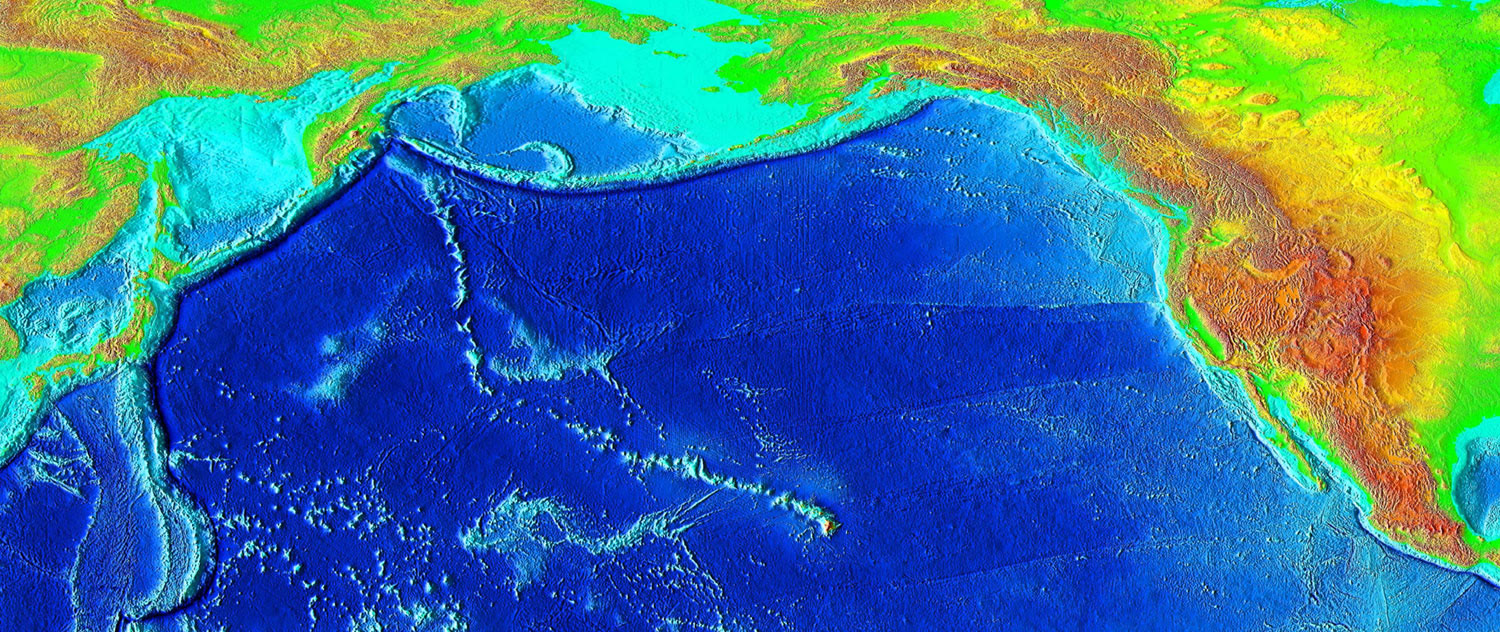
\includegraphics[width=\linewidth]{images/book2/g11-ngdc-hawaii-chain.jpg}

{\small Shaded relief of the floor of the North Pacific. The Hawaiian chain
runs from the island of Hawaii (bottom centre, brown) to the
west-north-west; at the bend it turns north into the Emperor seamounts, which
end at the trench along Kamchatka and the Aleutians. Image: National
Geophysical Data Center, NOAA (public domain).}
\end{omfigure}
% ledger: photo:g11-hawaii-chain

Potassium--argon dating of lavas from 37 volcanoes of the chain, collected on
the islands, dredged from the seamounts or drilled through their sediments,
gives their ages (graph below). Mauna Kea is about
\num{0.4} million years old, Kauai \num{5.1}, Midway \num{27.7}, and the
Suiko seamount, near the far end of the Emperor chain, \num{64.7}. The ages
grow with distance from Kilauea, the active volcano, as a \omterm{def:g11:plate-motions:hotspot-track}{hotspot track}
predicts.
% ledger: cd87:ages

\begin{omfigure}
\begin{tikzpicture}
\begin{axis}[ompt, width=0.82\linewidth, height=6.4cm, xmin=0, xmax=5000, ymin=0, ymax=70,
  xlabel={distance from Kilauea along the chain (\unit{km})}, ylabel={age (millions of years)},
  xticklabel style={/pgf/number format/set thousands separator={}},
  legend style={font=\scriptsize, at={(0.03,0.97)}, anchor=north west}, legend cell align=left]
% computed in figdata/grade-11/hawaii_chain.py; ledger: cd87:ages
\addplot[only marks, mark=o, mark size=1.6pt, omDef, error bars/.cd, y dir=both, y explicit]
  table[x=dist, y=age, y error=err] {figdata/out/grade-11-hawaii_chain-hawaiian.dat};
\addplot[only marks, mark=triangle, mark size=2pt, omProp, error bars/.cd, y dir=both, y explicit]
  table[x=dist, y=age, y error=err] {figdata/out/grade-11-hawaii_chain-emperor.dat};
\addplot[black, densely dashed, line width=0.6pt] table[x=dist, y=age] {figdata/out/grade-11-hawaii_chain-fit.dat};
\legend{Hawaiian chain, bend and Emperor chain, {line through the origin, \qty{9.1}{cm} a year}}
\draw[black!50, densely dotted] (axis cs:3400,0) -- (axis cs:3400,70);
\node[font=\scriptsize, anchor=south, rotate=90] at (axis cs:3400,8) {bend};
\node[font=\scriptsize, anchor=north west] at (axis cs:519,5.1) {Kauai};
\node[font=\scriptsize, anchor=south] at (axis cs:2432,30) {Midway};
\node[font=\scriptsize, anchor=south east] at (axis cs:4860,65.5) {Suiko};
\end{axis}
\end{tikzpicture}

{\small Age of the volcanoes of the Hawaiian--Emperor chain against their
distance from Kilauea, with the uncertainties of the ages. Along the
Hawaiian chain the points follow a straight line through the origin; beyond
the bend the ages grow faster with distance. Data: Clague and Dalrymple
(1987).}
\end{omfigure}

Along the Hawaiian chain, up to about \qty{3300}{km}, the points scatter
around a straight line through the origin. The line that best fits the 26
dated volcanoes of this part rises by one million years every
\qty{91}{km}: by \cref{prop:g11:plate-motions:hotspot}, the Pacific plate has
moved over the hotspot at about \qty{91}{km} per million years, \qty{9.1}{cm}
a year. The authors of the ages, fitting the whole chain in their own way,
found \qty{8.6}{cm} a year.
% ledger: cd87:ages (fit computed in hawaii_chain.py), cd87:rate

Beyond the bend, the ages grow faster with distance: along the Emperor
chain the plate moved more slowly, about \qty{6.5}{cm} a year on average
(best straight line through the nine dated seamounts). And the chain changes
direction. If the hotspot stayed in place, the bend records a change in the
direction of motion of the Pacific plate. Newer ages place
the beginning of the bend near the Kimmei seamount, about 50 million years
ago, at the same time as a reorganisation of the spreading ridges of the
Pacific and the first volcanoes of the island arcs along its western edge:
the plate changed course.
% ledger: cd87:ages (Emperor fit computed in hawaii_chain.py), sc06:bend

\section{The predictive power of the model}\label{sec:g11:plate-motions:predictive}

The plate model says that a few \omterm{def:g11:plate-motions:rigid-plate}{rigid plates} turn about their rotation poles,
and that almost everything happens at their boundaries. Its strength is that
measurements made by entirely different methods, over very different spans of
time, give the same answers.

\begin{itemize}
  \item \emph{Earthquakes and volcanoes} gather along the boundaries, and the
        kind of boundary predicts their kind: shallow earthquakes along the
        ridges, deep ones only near trenches (\cref{ch:g11:subduction-zones}).
  \item \emph{The ocean floor} is youngest along the ridges and older and
        older away from them, symmetrically on both sides
        (\cref{ch:g11:drift-to-spreading}).
  \item \emph{Mountain belts} rise where plates converge: India still moves
        toward Eurasia at about \qty{4.5}{cm} a year across the Himalaya,
        as computed from the rotation poles (\cref{ch:g12:mountain-building}).
  \item \emph{Speeds agree across methods}: the table below compares the
        speeds measured today by satellite positioning with those predicted
        by the rotation poles, whose \omterm{def:g11:drift-to-spreading:spreading-rate}{spreading rates} come mainly from
        magnetic stripes and average the motion over the last
        \num{0.8} to \num{3.2} million years, and with the speed recorded
        by a \omterm{def:g11:plate-motions:hotspot-track}{hotspot track} over tens of millions of years.
\end{itemize}
% ledger: nnr56:poles, nnr56:data (India-Eurasia computed in plate_velocities.py at 85 E 28 N)

\begin{center}
\small
\begin{tabular}{|l|c|c|}
\hline
what is measured & method & speed (\unit{cm} a year) \\ \hline
Mauna Kea, Pacific plate & satellite positioning, 30 years & 7.2 \\
Mauna Kea, Pacific plate & rotation pole & 6.9 \\
Wettzell, Eurasian plate & satellite positioning, 31 years & 2.6 \\
Wettzell, Eurasian plate & rotation pole & 2.3 \\
Pacific plate over the Hawaiian hotspot & volcano ages, 40 million years & 9.1 \\ \hline
\end{tabular}
\end{center}
% ledger: data:b2-ngl-gnss, nnr56:poles, cd87:ages (all computed in figdata/grade-11)

The rotation-pole speeds and the station speeds agree to within
\qty{0.3}{cm} a year, though the first average millions of years and the
second only decades: the plates move today as they have moved for millions of
years. The hotspot speed is larger: it is measured in another frame, that of
the hotspot itself, and over a far longer time.

One more pattern appears when the speeds of whole plates are compared. The
plates that move fastest, Cocos, Nazca, Pacific, Australian and Philippine
Sea, all have a long edge that sinks into the mantle at a trench; their mean
speeds average about \qty{6.5}{cm} a year. The plates without such
an edge, among them the Eurasian, North and South American, African and
Antarctic plates, move at about \qty{2.4}{cm} a year on average. This clue to
what drives the plates is taken up in \cref{ch:g11:subduction-zones}.
% ledger: nnr56:rms (means computed in plate_velocities.py)

\section{Exercises}

\begin{exercise}[$\star$]\label{exo:g11:plate-motions:1}
Define a \omterm{def:g11:plate-motions:rigid-plate}{rigid plate}. Where is the deformation of the \omterm{def:g11:lithosphere-asthenosphere:lithosphere}{lithosphere} gathered,
and which everyday seismic observation shows it?
\end{exercise}

\begin{exercise}[$\star$]\label{exo:g11:plate-motions:2}
The Mauna Kea station moves \qty{72}{mm} a year. Express this speed in
kilometres per million years. How far does the station move in 30 years? In
a million years?
\end{exercise}

\begin{exercise}[$\star$]\label{exo:g11:plate-motions:3}
In ten years, a station moved \qty{30}{cm} east and \qty{40}{cm} north. Find
its east and north speeds, its speed, and the angle its direction makes with
the north.
\end{exercise}

\begin{exercise}[$\star$]\label{exo:g11:plate-motions:4}
Define a \omterm{def:g11:plate-motions:hotspot-track}{hotspot track}. Along the Hawaiian chain, where is the youngest
volcano, and in which direction do the ages increase? What does that tell
about the direction in which the Pacific plate moves?
\end{exercise}

\begin{exercise}[$\star$]\label{exo:g11:plate-motions:5}
Kauai lies \qty{519}{km} from Kilauea along the chain, and its oldest lavas
are \num{5.1} million years old. Assuming the hotspot is fixed, at what
average speed has the plate carried it, in kilometres per million years and
in centimetres a year?
\end{exercise}

\begin{exercise}[$\star\star$]\label{exo:g11:plate-motions:6}
In the graph of the two station series, the Wettzell station moved about
\qty{63}{cm} east and \qty{48}{cm} north in 31 years. Find its east and north
speeds, its speed, and its direction. Compare its speed with that of Mauna
Kea.
\end{exercise}

\begin{exercise}[$\star\star$]\label{exo:g11:plate-motions:7}
In Iceland, at \ang{64.5} North and \ang{18} West, the rotation poles give
the North American plate the velocity $(-10.5, +20.6)$ and the Eurasian
plate $(+7.7, +16.3)$, in millimetres a year (east, north). (1) Find the
velocity of North America relative to Eurasia, its speed and its direction.
(2) What is this speed for the ridge that crosses Iceland? (3) Compare with
the rate of \qty{2}{cm} a year often quoted for the North Atlantic.
\end{exercise}

\begin{exercise}[$\star\star$]\label{exo:g11:plate-motions:8}
The Pacific plate turns by \ang{0.651} per million years. (1) Find the speed
of a point \ang{90} from its rotation pole, in centimetres a year. (2) And of
a point \ang{30} from the pole? (3) Where on a plate is the speed zero? Can
the speed of a whole plate be given by one number?
\end{exercise}

\begin{exercise}[$\star\star$]\label{exo:g11:plate-motions:9}
North of the Himalaya, at \ang{28} North and \ang{85} East, the rotation poles
give the Indian plate the velocity $(+40.6, +38.6)$ and the Eurasian plate
$(+24.0, -3.3)$, in millimetres a year (east, north). (1) Find the velocity of
India relative to Eurasia, its speed and its direction. (2) If it stayed the
same, by how much would the two plates converge in 10 million years?
\end{exercise}

\begin{exercise}[$\star\star$]\label{exo:g11:plate-motions:10}
Necker lies \qty{1058}{km} from Kilauea and is \num{10.3} million years old;
Midway lies \qty{2432}{km} away and is \num{27.7} million years old. Find the
speed of the plate over the hotspot between the times the two volcanoes were
built. Compare with \qty{9.1}{cm} a year.
\end{exercise}

\begin{exercise}[$\star\star$]\label{exo:g11:plate-motions:11}
At a point, plate $A$ moves \qty{3}{cm} a year east relative to plate $B$,
and plate $B$ moves \qty{4}{cm} a year north relative to plate $C$.
(1) Draw the velocity triangle and find the velocity of $A$ relative to $C$:
speed and direction. (2) What is the velocity of $C$ relative to $A$?
\end{exercise}

\begin{exercise}[$\star\star\star$]\label{exo:g11:plate-motions:12}
Mauna Kea lies \qty{54}{km} from Kilauea and is \num{0.375} million years
old. (1) What speed does it give for the plate? (2) A volcano is some tens of
kilometres across, and it grows for several hundred thousand years. Suppose
its distance from the hotspot is uncertain by \qty{25}{km}: between which
values does the speed then lie? (3) Explain why young volcanoes close to the
hotspot give a poor estimate of the speed, and why the volcanoes far from it
are better.
\end{exercise}

\begin{exercise}[$\star\star\star$]\label{exo:g11:plate-motions:13}
The monthly positions of a station scatter by about \qty{5}{mm} about their
straight line. A motion is clearly seen once it exceeds ten times the scatter.
(1) How long must one measure to see clearly the motion of the Mauna Kea
station, \qty{72}{mm} a year? (2) And a motion of \qty{5}{mm} a year, as
across a slowly deforming region inside a continent? (3) Why were plate
speeds measured from magnetic stripes long before satellites could measure
them?
\end{exercise}

\begin{exercise}[$\star\star\star$]\label{exo:g11:plate-motions:14}
On the Mid-Atlantic Ridge at \ang{30} South (\ang{13.5} West), the rotation
poles give the South American plate the velocity $(-4.9, +11.0)$ and the
African plate $(+27.1, +17.9)$, in millimetres a year (east, north).
(1) Find the velocity of South America relative to Africa, its speed and its
direction. (2) Deduce the full and the half \omterm{def:g11:drift-to-spreading:spreading-rate}{spreading rates} of the ridge.
(3) The sediments of the South Atlantic gave a half rate of about \qty{1.9}{cm}
a year averaged over the last 66 million years
(\cref{ch:g11:drift-to-spreading}). Compare, and suggest what the difference
may mean.
\end{exercise}

\begin{exercise}[$\star\star\star$]\label{exo:g11:plate-motions:15}
A station moves steadily \qty{20}{mm} a year east. Exactly halfway through
ten years of measurement, an earthquake shifts it suddenly by \qty{50}{mm}
toward the west. (1) Sketch its east position against time. (2) What speed
would one find from the first and the last positions alone? (3) What speed do
the two halves of the series give, each on its own? (4) How should a
geodesist deal with such a jump?
\end{exercise}

\section{Problem: Reading the Hawaiian--Emperor Chain}

\begin{problem}[{Weekend problem --- a plate's speed written in volcanoes}]
\label{pb:g11:plate-motions:1}
% values from Clague and Dalrymple 1987, Table 1.4 (ledger cd87:ages); fits computed in
% figdata/grade-11/hawaii_chain.py (v_hawaiian 91.2, v_emperor_free 64.6); bend sc06:bend;
% MKEA rates data:b2-ngl-gnss
The table gives the distance from Kilauea, measured along the chain, and the
potassium--argon age of thirteen volcanoes of the Hawaiian--Emperor chain.
Kilauea is the active volcano over the hotspot; the bend lies between Abbott
and Daikakuji.

\begin{center}
\small
\begin{tabular}{|l|c|c||l|c|c|}
\hline
volcano & distance (\unit{km}) & age (\unit{Ma}) & volcano & distance (\unit{km}) & age (\unit{Ma}) \\ \hline
Mauna Kea & 54 & 0.375 & Abbott & 3280 & 38.7 \\ \hline
Kauai & 519 & 5.1 & Daikakuji & 3493 & 42.4 \\ \hline
Nihoa & 780 & 7.2 & Koko (south) & 3758 & 48.1 \\ \hline
Necker & 1058 & 10.3 & Ojin & 4102 & 55.2 \\ \hline
Laysan & 1818 & 19.9 & Nintoku & 4452 & 56.2 \\ \hline
Midway & 2432 & 27.7 & Suiko (centre) & 4860 & 64.7 \\ \hline
Colahan & 3128 & 38.6 & & & \\ \hline
\end{tabular}
\end{center}

\medskip
\noindent\textbf{Part I --- Ages and distances.}
\begin{enumerate}
  \item Which volcano of the table is the youngest, and which the oldest? How
        do the ages change along the chain?
  \item Show that a distance in kilometres divided by an age in millions of
        years is a speed in millimetres a year.
  \item Compute the average speed $d/t$ given by Kauai.
  \item Compute $d/t$ for Necker, Laysan, Midway, Colahan and Abbott.
  \item Plot the age against the distance for the eight volcanoes of the
        table that lie before the bend. Do the points lie close to a straight line through
        the origin?
\end{enumerate}

\medskip
\noindent\textbf{Part II --- The plate's speed over the hotspot.}
\begin{enumerate}[resume]
  \item Explain why, for a fixed hotspot and a plate moving at a steady
        speed $v$, the age $t$ and the distance $d$ satisfy $t = d/v$.
  \item Compute the mean of the five speeds of question~4.
  \item The straight line through the origin that best fits all 26 dated
        volcanoes of the Hawaiian chain gives \qty{91}{km} per million years.
        Compare with question~7.
  \item At this speed, how long would the plate take to carry Kauai from the
        hotspot to its present place? Compare with its age.
  \item In which direction does the Pacific plate move over the hotspot?
\end{enumerate}

\medskip
\noindent\textbf{Part III --- The bend.}
\begin{enumerate}[resume]
  \item Compute the average speed of the plate between the times Daikakuji
        and Suiko (centre) were built.
  \item The best straight line through the nine dated volcanoes from
        Daikakuji onward gives \qty{65}{km} per million years. Compare with
        the speed along the Hawaiian chain.
  \item Newer ages place the start of the bend near the Kimmei
        seamount, \qty{3668}{km} from Kilauea, about 50 million years ago.
        What average speed does that give for the whole Hawaiian chain?
        Compare with \qty{91}{km} per million years, and explain why both can
        be right.
  \item If the hotspot stayed fixed, what does the bend record about the
        Pacific plate?
  \item The newer dating found large changes of speed along the Emperor chain
        with little change in its direction. Explain why the direction of a
        chain and the spacing of its ages are two independent pieces of
        information.
\end{enumerate}

\medskip
\noindent\textbf{Part IV --- Comparison with today's satellite measurement.}
\begin{enumerate}[resume]
  \item The Mauna Kea station moves $\qty{-63.2}{mm}$ a year east and
        $\qty{+34.5}{mm}$ a year north. Find its speed and its direction.
  \item The Hawaiian chain runs from Kilauea toward the west-north-west. Is
        the direction of the station consistent with it?
  \item The station gives \qty{7.2}{cm} a year, the chain \qty{9.1}{cm} a year.
        Give two reasons why the two numbers need not be equal.
  \item At \qty{91}{km} per million years, how long will the plate take to
        carry Mauna Kea another \qty{100}{km} away from the hotspot?
  \item Conclude: at what speed has the Pacific plate moved over the Hawaiian
        hotspot during the last 40 million years?
\end{enumerate}
\end{problem}
